\documentclass[aspectratio=169,spanish,xcolor=table]{beamer}
\usepackage{iftex}
\ifPDFTeX
  \usepackage[utf8]{inputenc}
  \usepackage[T1]{fontenc}
\fi
\usepackage[spanish,es-tabla,es-noshorthands]{babel}
\usepackage{helvet}
\renewcommand{\familydefault}{\sfdefault}
\usepackage{tikz,pgfplots,array,booktabs,ragged2e}
\pgfplotsset{compat=1.18}
\usetikzlibrary{arrows.meta,positioning,calc,shapes.geometric,fit}

\definecolor{iiiepeNavy}{HTML}{163B5C}
\definecolor{iiiepeBlue}{HTML}{1F6F9F}
\definecolor{iiiepeAqua}{HTML}{20B7A8}
\definecolor{iiiepeOrange}{HTML}{F28C28}
\definecolor{iiiepePaper}{HTML}{F6F8F7}
\definecolor{iiiepeInk}{HTML}{1E2A32}
\definecolor{iiiepePale}{HTML}{EEF5F8}
\definecolor{iiiepeMint}{HTML}{E7F6F4}
\definecolor{iiiepeWarm}{HTML}{FFF3E6}

\usetheme{default}
\usecolortheme{default}
\setbeamertemplate{navigation symbols}{}
\setbeamercolor{normal text}{fg=iiiepeInk,bg=white}
\setbeamercolor{structure}{fg=iiiepeNavy}
\setbeamercolor{frametitle}{fg=white,bg=iiiepeNavy}
\setbeamercolor{block title}{fg=white,bg=iiiepeBlue}
\setbeamercolor{block body}{fg=iiiepeInk,bg=iiiepePale}
\setbeamercolor{item}{fg=iiiepeOrange}

\setbeamertemplate{frametitle}{%
  \nointerlineskip%
  \begin{beamercolorbox}[wd=\paperwidth,ht=0.95cm,dp=0.22cm,leftskip=0.45cm,rightskip=0.45cm]{frametitle}%
    \begin{minipage}[c]{13.2cm}\usebeamerfont{frametitle}\large\bfseries\insertframetitle\end{minipage}%
    \hfill\begin{minipage}[c]{1.6cm}\raggedleft\includegraphics[height=0.56cm]{img/iiiepe/logo-iiiepe-blanco.png}\end{minipage}%
  \end{beamercolorbox}%
}

\setbeamertemplate{footline}{%
  \leavevmode%
  \hbox{%
    \begin{beamercolorbox}[wd=.78\paperwidth,ht=0.5cm,dp=0.18cm,leftskip=0.45cm]{frametitle}%
      \scriptsize\color{white}M. de la Cruz Muñoz · MAEM · Matrícula 00874 · SD26 · Actividad 9 · Infografía Sawyer%
    \end{beamercolorbox}%
    \begin{beamercolorbox}[wd=.22\paperwidth,ht=0.5cm,dp=0.18cm,rightskip=0.45cm]{frametitle}%
      \hfill\scriptsize\color{white}\insertframenumber{} / \inserttotalframenumber%
    \end{beamercolorbox}%
  }%
  \vskip0pt%
}

\newcommand{\Pill}[2]{%
  \tikz[baseline=(x.base)]{\node[rounded corners=3pt,fill=#1!14,draw=#1!75!black,thick,inner xsep=6pt,inner ysep=4pt,align=center] (x) {\scriptsize\bfseries #2};}%
}

\title{Ciencias del Aprendizaje: Infografía y Análisis de R. Keith Sawyer (2008)}
\subtitle{Actividad 9 · Sesión 3b · Complemento Infográfico (Módulo 51440 / 51436)}
\author{Mtro. Martín Jonathan de la Cruz Muñoz · Matrícula 00874}
\institute{IIIEPE · Maestría en Aprendizaje y Enseñanza de las Matemáticas · Grupo A}
\date{19 de noviembre de 2026}

% Motor visual editorial para infografías en LaTeX/TikZ (Cohorte SD26 · IIIEPE MAEM)
\definecolor{infNavy}{HTML}{1A4F7A}
\definecolor{infBlueLight}{HTML}{DCEBF7}
\definecolor{infBlueCard}{HTML}{EDF5FC}
\definecolor{infBlueAccent}{HTML}{2775B3}

\definecolor{infGreen}{HTML}{1E6B43}
\definecolor{infGreenLight}{HTML}{DCF2E4}
\definecolor{infGreenCard}{HTML}{EEF9F2}
\definecolor{infGreenAccent}{HTML}{2A935B}

\definecolor{infOrange}{HTML}{C45522}
\definecolor{infOrangeLight}{HTML}{FDE6D8}
\definecolor{infOrangeCard}{HTML}{FEF3EB}
\definecolor{infOrangeAccent}{HTML}{DE6A31}

\definecolor{infInk}{HTML}{1E2932}
\definecolor{infPaper}{HTML}{F8FAFC}
\definecolor{infBorder}{HTML}{C9D6E2}

\tikzset{
  pics/inf_target/.style={code={
    \draw (0,0) circle (.78);
    \draw (0,0) circle (.46);
    \fill (0,0) circle (.16);
    \draw[line width=1.4pt] (.42,.42) -- (.95,.95);
    \draw (.62,.95) -- (.95,.95) -- (.95,.62);
  }},
  pics/inf_doc/.style={code={
    \draw[rounded corners=1.2pt] (-.65,-.85) rectangle (.65,.85);
    \draw (-.38,.42) -- (.38,.42);
    \draw (-.38,.08) -- (.38,.08);
    \draw (-.38,-.26) -- (.38,-.26);
    \draw (-.38,-.58) -- (.12,-.58);
  }},
  pics/inf_key/.style={code={
    \draw (-.38,.12) circle (.38);
    \draw[line width=1.6pt] (0,.12) -- (.92,.12);
    \draw[line width=1.5pt] (.58,.12) -- (.58,-.28);
    \draw[line width=1.5pt] (.85,.12) -- (.85,-.20);
  }},
  pics/inf_bulb/.style={code={
    \draw (-.32,-.28) .. controls (-.58,-.05) and (-.62,.45) .. (0,.65)
      .. controls (.62,.45) and (.58,-.05) .. (.32,-.28) -- cycle;
    \draw (-.26,-.48) -- (.26,-.48);
    \draw (-.20,-.70) -- (.20,-.70);
    \draw (0,.82) -- (0,1.02) (.68,.55) -- (.84,.68) (-.68,.55) -- (-.84,.68);
  }},
  pics/inf_gear/.style={code={
    \draw (0,0) circle (.46);
    \draw (0,0) circle (.18);
    \foreach \a in {0,45,...,315}{
      \draw[line width=2.2pt] (\a:.46) -- (\a:.76);
    }
  }},
  pics/inf_personas/.style={code={
    \draw (0,.48) circle (.24);
    \draw (-.64,.25) circle (.19) (.64,.25) circle (.19);
    \draw (-.42,-.72) -- (-.42,-.18) .. controls (-.42,.18) and (.42,.18) .. (.42,-.18) -- (.42,-.72);
    \draw (-.95,-.66) -- (-.95,-.24) .. controls (-.95,.02) and (-.56,.02) .. (-.48,-.22);
    \draw (.48,-.22) .. controls (.56,.02) and (.95,.02) .. (.95,-.24) -- (.95,-.66);
  }},
  pics/inf_autonomia/.style={code={
    \draw[dashed] (0,0) circle (.88);
    \draw (0,.42) circle (.24);
    \draw (-.38,-.58) -- (-.38,-.15) .. controls (-.38,.18) and (.38,.18) .. (.38,-.15) -- (.38,-.58);
  }},
  pics/inf_alerta/.style={code={
    \draw[rounded corners=1.5pt] (0,.85) -- (-.92,-.72) -- (.92,-.72) -- cycle;
    \draw[line width=1.6pt] (0,.30) -- (0,-.22);
    \fill (0,-.48) circle (.09);
  }},
  pics/inf_balanza/.style={code={
    \draw (0,-.75) -- (0,.72);
    \draw (-.50,-.75) -- (.50,-.75);
    \draw (-.75,.48) -- (.75,.48);
    \draw (-.75,.48) -- (-.95,-.05) -- (-.55,-.05) -- cycle;
    \draw (.75,.48) -- (.55,-.05) -- (.95,-.05) -- cycle;
  }},
  pics/inf_cerebro/.style={code={
    \draw (-.1,.62) .. controls (-.72,.68) and (-.95,.15) .. (-.68,-.28)
      .. controls (-.82,-.65) and (-.28,-.75) .. (0,-.52);
    \draw (.1,.62) .. controls (.72,.68) and (.95,.15) .. (.68,-.28)
      .. controls (.82,-.65) and (.28,-.75) .. (0,-.52);
    \draw (0,.65) -- (0,-.52);
    \draw (-.45,.18) -- (-.15,.05) (.45,.18) -- (.15,.05) (-.42,-.22) -- (-.12,-.18);
  }},
  pics/inf_construccion/.style={code={
    \draw (0,0) circle (.45);
    \draw (0,0) circle (.16);
    \foreach \a in {0,60,...,300}{
      \draw[line width=2pt] (\a:.45) -- (\a:.74);
    }
    \draw (.62,.62) circle (.22);
  }},
  pics/inf_dialogo/.style={code={
    \draw[rounded corners=2pt] (-.92,.78) -- (.48,.78) -- (.48,-.04)
      -- (-.32,-.04) -- (-.68,-.40) -- (-.68,-.04) -- (-.92,-.04) -- cycle;
    \draw[rounded corners=1.5pt] (.15,-.18) -- (.92,-.18) -- (.92,-.76)
      -- (.68,-.76) -- (.68,-.98) -- (.38,-.76) -- (.15,-.76) -- cycle;
    \draw (-.64,.48) -- (.22,.48) (-.64,.22) -- (.06,.22);
  }},
  pics/inf_grafica/.style={code={
    \draw (-.88,.85) -- (-.88,-.75) -- (.92,-.75);
    \fill (-.62,-.75) rectangle (-.32,-.10);
    \fill (-.15,-.75) rectangle (.15,.25);
    \fill (.32,-.75) rectangle (.62,.68);
  }},
  pics/inf_lupa/.style={code={
    \draw (-.18,.22) circle (.54);
    \draw[line width=1.8pt] (.22,-.18) -- (.88,-.84);
    \draw (-.48,.28) .. controls (-.44,.50) and (-.26,.58) .. (-.06,.56);
  }},
  pics/inf_escuela/.style={code={
    \draw (-.85,-.75) rectangle (.85,.25);
    \draw (-1.0,.25) -- (0,.92) -- (1.0,.25);
    \draw (-.20,-.75) rectangle (.20,-.10);
    \draw (-.64,-.08) rectangle (-.38,.12);
    \draw (.38,-.08) rectangle (.64,.12);
    \draw (0,.52) circle (.12);
  }},
  pics/inf_andamio/.style={code={
    \draw (-.82,-.75) -- (-.82,.75) (.82,-.75) -- (.82,.75);
    \draw (-.82,-.30) -- (.82,-.30) (-.82,.22) -- (.82,.22) (-.82,.72) -- (.82,.72);
    \draw (-.82,-.30) -- (.82,.22) (.82,-.30) -- (-.82,.22);
    \fill[draw=none] (0,.84) circle (.10);
  }},
  pics/inf_libro/.style={code={
    \draw (0,-.68) -- (0,.58);
    \draw (0,.58) .. controls (-.34,.85) and (-.68,.85) .. (-.96,.64)
      -- (-.96,-.58) .. controls (-.58,-.42) and (-.26,-.45) .. (0,-.68);
    \draw (0,.58) .. controls (.34,.85) and (.68,.85) .. (.96,.64)
      -- (.96,-.58) .. controls (.58,-.42) and (.26,-.45) .. (0,-.68);
    \draw (-.72,.28) -- (-.24,.14) (-.72,-.04) -- (-.24,-.18);
    \draw (.24,.14) -- (.72,.28) (.24,-.18) -- (.72,-.04);
  }}
}

\newcommand{\InfIcon}[3][0.30]{%
  \begin{tikzpicture}[x=#1cm,y=#1cm,baseline=-0.12cm]
    \path[use as bounding box] (-1.05,-1.05) rectangle (1.05,1.05);
    \pic[draw=#3,fill=#3,line width=1.15pt,line cap=round,line join=round] {inf_#2};
  \end{tikzpicture}%
}

\newcommand{\InfIconOutline}[3][0.30]{%
  \begin{tikzpicture}[x=#1cm,y=#1cm,baseline=-0.12cm]
    \path[use as bounding box] (-1.05,-1.05) rectangle (1.05,1.05);
    \pic[draw=#3,line width=1.15pt,line cap=round,line join=round] {inf_#2};
  \end{tikzpicture}%
}

\newcommand{\InfPillBar}[5]{%
  % #1=x, #2=y, #3=colorDark, #4=colorLight, #5=iconName, macro uses text via helper? Wait: pass #6=Title
}

% Medallón + Píldora horizontal de sección (ancho 7.75cm dentro de columna 8.15cm)
\newcommand{\InfSectionBar}[6]{%
  % (#1,#2)=origen izq, #3=accentColor, #4=lightColor, #5=icon, #6=Title
  \fill[#4,rounded corners=7pt] ({#1+0.25},{#2-0.46}) rectangle ({#1+7.75},{#2-0.02});
  \node[anchor=west,font=\fontsize{8.1}{9.5}\selectfont\bfseries\color{#3}] at ({#1+0.78},{#2-0.24}) {#6};
  \filldraw[fill=#3,draw=white,line width=1.4pt] ({#1+0.34},{#2-0.24}) circle (0.28cm);
  \node[inner sep=0pt] at ({#1+0.34},{#2-0.24}) {\InfIconOutline[0.18]{#5}{white}};
}

% Mini-tarjeta cuadrada de concepto clave (ancho 1.83cm x alto 2.18cm)
\newcommand{\InfConceptCard}[6]{%
  % #1=x, #2=y_top, #3=accentColor, #4=cardBg, #5=icon, #6=Title\\desc
  \draw[fill=#4,draw=#3!35!white,line width=0.6pt,rounded corners=4pt] ({#1},{#2-2.18}) rectangle ({#1+1.83},{#2});
  \node[inner sep=0pt] at ({#1+0.915},{#2-0.52}) {\InfIconOutline[0.32]{#5}{#3}};
  \node[anchor=north,text width=1.68cm,align=center,font=\fontsize{5.6}{6.8}\selectfont\color{infInk},inner sep=1pt] at ({#1+0.915},{#2-0.96}) {#6};
}

% Viñeta con círculo de color (Tesis / Aportes principales)
\newcommand{\InfBullet}[4]{%
  % #1=x, #2=y_top, #3=accentColor, #4=texto
  \fill[#3] ({#1+0.12},{#2-0.14}) circle (0.065cm);
  \node[anchor=north west,text width=7.35cm,align=left,font=\fontsize{6.3}{7.6}\selectfont\color{infInk},inner sep=0pt] at ({#1+0.28},{#2}) {#4};
}

% Viñeta con círculo Check ✓ (Implicaciones para la práctica)
\newcommand{\InfCheck}[4]{%
  % #1=x, #2=y_top, #3=accentColor, #4=texto
  \fill[#3] ({#1+0.14},{#2-0.15}) circle (0.125cm);
  \draw[white,line width=0.95pt,line cap=round,line join=round] ({#1+0.075},{#2-0.16}) -- ({#1+0.125},{#2-0.21}) -- ({#1+0.215},{#2-0.095});
  \node[anchor=north west,text width=7.28cm,align=left,font=\fontsize{6.3}{7.6}\selectfont\color{infInk},inner sep=0pt] at ({#1+0.34},{#2}) {#4};
}

\begin{document}

\begin{frame}[plain]
  \begin{tikzpicture}[remember picture,overlay]
    \fill[iiiepeNavy] (current page.north west) rectangle ([xshift=10.3cm]current page.south west);
    \fill[iiiepeBlue] ([xshift=10.3cm]current page.north west) rectangle (current page.south east);
    \fill[iiiepeOrange] ([xshift=0.8cm,yshift=-6.45cm]current page.north west) rectangle ([xshift=9.3cm,yshift=-6.53cm]current page.north west);
    \node[anchor=north west,text width=8.7cm,align=left] at ([xshift=0.8cm,yshift=-1.15cm]current page.north west) {%
      {\color{iiiepeAqua!45!white}\small\bfseries MAESTRÍA EN APRENDIZAJE Y ENSEÑANZA DE LAS MATEMÁTICAS · SD26\par}%
      \vspace{0.35cm}
      {\color{white}\Large\bfseries \inserttitle\par}%
      \vspace{0.25cm}
      {\color{white!90}\normalsize \insertsubtitle\par}%
    };
    \node[anchor=south west,text width=8.7cm,align=left] at ([xshift=0.8cm,yshift=0.75cm]current page.south west) {%
      {\color{white}\normalsize\bfseries Mtro. Martín Jonathan de la Cruz Muñoz\par}%
      {\color{white!85}\scriptsize Matrícula 00874 · martin.delacruz@campus.iiiepe.edu.mx\par}%
      {\color{iiiepeAqua!35!white}\scriptsize Monterrey, Nuevo León · 19 de noviembre de 2026\par}%
    };
    \node[anchor=center,text width=5.0cm,align=center] at ([xshift=13.15cm,yshift=-4.5cm]current page.north west) {%
      \includegraphics[width=3.6cm]{img/iiiepe/logo-iiiepe-blanco.png}\par\vspace{0.45cm}%
      {\color{white}\large\bfseries IIIEPE\par}%
      \vspace{0.1cm}%
      {\color{white!85}\scriptsize Fundamentos para la enseñanza\\y el aprendizaje I\par}%
    };
  \end{tikzpicture}
\end{frame}
\begin{frame}{Propósito: Superar el Instruccionismo con Ciencias del Aprendizaje}
  \begin{block}{Pregunta orientadora · R. Keith Sawyer (2008)}
    ¿Por qué las escuelas heredadas de la era industrial resultan insuficientes para formar analistas simbólicos y profesionales capaces de modelar, decidir e innovar?
  \end{block}
  \vspace{0.25cm}
  \begin{columns}[T]
    \column{0.48\textwidth}
      \begin{block}{Modelo estándar (Instruccionismo)}
        \begin{itemize}\scriptsize
          \item Conocimiento reducido a hechos aislados y rutinas.
          \item Secuencia rígida definida por adultos expertos.
          \item Evaluación sumativa centrada en memoria superficial.
        \end{itemize}
      \end{block}
    \column{0.48\textwidth}
      \begin{block}{Economía del conocimiento y aula profunda}
        \begin{itemize}\scriptsize
          \item Integración conceptual transferible a situaciones nuevas.
          \item Prácticas auténticas ancladas a disciplinas reales.
          \item Trabajo colaborativo con herramientas y diálogo experto.
        \end{itemize}
      \end{block}
  \end{columns}
\end{frame}

\begin{frame}[plain]
  \centering
  \resizebox{0.97\textwidth}{!}{\begin{tikzpicture}[x=1cm,y=1cm]
  \fill[infPaper] (-0.30,-17.05) rectangle (25.45,0.20);

  % COL 1: INSTRUCCIONISMO VS ECONOMIA DEL CONOCIMIENTO
  \draw[fill=white,draw=infGreen,line width=1.1pt,rounded corners=7pt] (0.0,-15.72) rectangle (8.15,0.0);
  \fill[infGreen,rounded corners=6pt] (0.0,-2.48) rectangle (8.15,0.0);
  \fill[infGreen] (0.0,-2.48) rectangle (8.15,-2.00);
  \node[anchor=north west,text width=5.45cm,align=left,inner sep=0pt] at (0.28,-0.22) {%
    {\color{white}\fontsize{11.5}{13.5}\selectfont\bfseries Keith Sawyer (I)\par}\vspace{2pt}%
    {\color{white!90}\fontsize{7.3}{8.6}\selectfont\bfseries Crisis del instruccionismo\\y economía creativa\par}\vspace{3pt}%
    {\colorbox{infGreenAccent}{\color{white}\fontsize{6.3}{7.3}\selectfont\bfseries\ Eje 1 · Modelo Estándar vs. Siglo XXI \ }}%
  };
  \node[inner sep=0pt] at (6.92,-1.24) {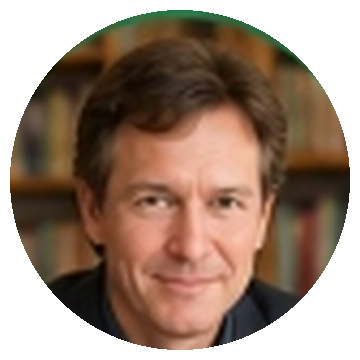
\includegraphics[width=2.06cm]{img_infografia/sawyer_photo.png}};

  \fill[infGreenLight] (0.12,-3.04) rectangle (8.03,-2.56);
  \node[font=\fontsize{6.9}{8.0}\selectfont\bfseries\color{infGreen}] at (4.075,-2.80) {Mejorando el aprendizaje: ciencias del aprendizaje (2008)};

  \InfSectionBar{0.20}{-3.16}{infGreen}{infGreenLight}{target}{Idea central del eje}
  \node[anchor=north west,text width=7.65cm,align=left,font=\fontsize{6.6}{8.0}\selectfont\color{infInk},inner sep=0pt] at (0.25,-3.74) {%
    La escuela fabril surgió sin investigación empírica sobre cómo aprendemos; hoy la economía creativa requiere «analistas simbólicos» capaces de modelar, innovar y transferir ideas.%
  };

  \InfSectionBar{0.20}{-4.86}{infGreen}{infGreenLight}{key}{Conceptos clave}
  \InfConceptCard{0.20}{-5.44}{infGreen}{infGreenCard}{alerta}{\textbf{Instruccionismo}\\Transmisión lineal fabril (Papert).}
  \InfConceptCard{2.17}{-5.44}{infGreen}{infGreenCard}{cerebro}{\textbf{Analista simbólico}\\Creación e ingenio conceptual.}
  \InfConceptCard{4.14}{-5.44}{infGreen}{infGreenCard}{escuela}{\textbf{Saber situado}\\Sujeto, herramientas y contexto.}
  \InfConceptCard{6.11}{-5.44}{infGreen}{infGreenCard}{construccion}{\textbf{Práctica experta}\\Participar en quehacer científico.}

  \InfSectionBar{0.20}{-7.78}{infGreen}{infGreenLight}{bulb}{Aportes principales}
  \InfBullet{0.22}{-8.38}{infGreen}{Supuesto tradicional: conocer es acumular hechos sueltos y procedimientos cuya ordenación definieron adultos.}
  \InfBullet{0.22}{-9.04}{infGreen}{Las ciencias del aprendizaje unen psicología cognitiva, computación, neurociencias, sociología y diseño.}
  \InfBullet{0.22}{-9.70}{infGreen}{El conocimiento no es estructura estática dentro del cráneo: emerge en actividad social situada.}
  \InfBullet{0.22}{-10.36}{infGreen}{Formar técnicos e ingenieros exige practicar modelos y explicaciones auténticas, no memoria repetitiva.}

  \InfSectionBar{0.20}{-11.12}{infGreen}{infGreenLight}{gear}{Implicaciones en Matemáticas}
  \InfCheck{0.22}{-11.72}{infGreen}{Sustituir series repetitivas por desafíos de modelación real.}
  \InfCheck{0.22}{-12.26}{infGreen}{Conectar variables simbólicas con mediciones de taller.}
  \InfCheck{0.22}{-12.80}{infGreen}{Reconocer límites de aplicación física de cada fórmula.}
  \InfCheck{0.22}{-13.34}{infGreen}{Actuar el aula como laboratorio interdisciplinario activo.}

  \fill[infGreenLight,rounded corners=5pt] (0.20,-15.52) rectangle (7.95,-14.05);
  \node[text width=7.35cm,align=center,font=\fontsize{6.6}{8.1}\selectfont\color{infGreen}] at (4.075,-14.78) {%
    \textbf{\textit{«El modelo estándar preparó para la fábrica, pero limita la comprensión profunda hoy necesaria.»}}\\
    {\scriptsize — Eje histórico · Sawyer (2008)}%
  };

  % COL 2: HALLAZGOS COGNITIVOS, ARTICULACION Y ANDAMIAJE
  \draw[fill=white,draw=infNavy,line width=1.1pt,rounded corners=7pt] (8.50,-15.72) rectangle (16.65,0.0);
  \fill[infNavy,rounded corners=6pt] (8.50,-2.48) rectangle (16.65,0.0);
  \fill[infNavy] (8.50,-2.48) rectangle (16.65,-2.00);
  \node[anchor=north west,text width=5.45cm,align=left,inner sep=0pt] at (8.78,-0.22) {%
    {\color{white}\fontsize{11.5}{13.5}\selectfont\bfseries Keith Sawyer (II)\par}\vspace{2pt}%
    {\color{white!90}\fontsize{7.3}{8.6}\selectfont\bfseries Hallazgos cognitivos,\\articulación y andamiaje\par}\vspace{3pt}%
    {\colorbox{infBlueAccent}{\color{white}\fontsize{6.3}{7.3}\selectfont\bfseries\ Eje 2 · Mecanismos del Aprendizaje \ }}%
  };
  \node[inner sep=0pt] at (15.42,-1.24) {
\includegraphics[width=2.06cm]{img_infografia/sawyer_illus.png}};

  \fill[infBlueLight] (8.62,-3.04) rectangle (16.53,-2.56);
  \node[font=\fontsize{6.9}{8.0}\selectfont\bfseries\color{infNavy}] at (12.575,-2.80) {Saberes previos, pensamiento visible y scaffolding efectivo};

  \InfSectionBar{8.70}{-3.16}{infNavy}{infBlueLight}{target}{Idea central del eje}
  \node[anchor=north west,text width=7.65cm,align=left,font=\fontsize{6.6}{8.0}\selectfont\color{infInk},inner sep=0pt] at (8.75,-3.74) {%
    Comprender profundamente ocurre al integrar hechos en redes conceptuales, explicitar «matemáticas ingenuas», externalizar razonamientos en voz alta y graduar el andamiaje docente.%
  };

  \InfSectionBar{8.70}{-4.86}{infNavy}{infBlueLight}{key}{Conceptos clave}
  \InfConceptCard{8.70}{-5.44}{infNavy}{infBlueCard}{lupa}{\textbf{Ideas ingenuas}\\Teorías previas del aprendiz.}
  \InfConceptCard{10.67}{-5.44}{infNavy}{infBlueCard}{dialogo}{\textbf{Articulación}\\Pensar en voz alta y explicar.}
  \InfConceptCard{12.64}{-5.44}{infNavy}{infBlueCard}{target}{\textbf{Metacognición}\\Monitorear el propio camino.}
  \InfConceptCard{14.61}{-5.44}{infNavy}{infBlueCard}{andamio}{\textbf{Andamiaje}\\Guía que se retira con autonomía.}

  \InfSectionBar{8.70}{-7.78}{infNavy}{infBlueLight}{bulb}{Aportes principales}
  \InfBullet{8.72}{-8.38}{infNavy}{Los aprendices no llegan como vasos vacíos: su error suele expresar una teoría intuitiva coherente que debe aflorar.}
  \InfBullet{8.72}{-9.04}{infNavy}{La pericia experta combina esquemas ricos, adaptación improvisada en el espacio del problema y reflexión.}
  \InfBullet{8.72}{-9.70}{infNavy}{Articulación y comprensión se refuerzan mutuamente: explicar a otros acelera el dominio conceptual.}
  \InfBullet{8.72}{-10.36}{infNavy}{El buen andamiaje da pistas y preguntas detonadoras sin resolver la tarea en lugar del estudiante.}

  \InfSectionBar{8.70}{-11.12}{infNavy}{infBlueLight}{gear}{Implicaciones en Matemáticas}
  \InfCheck{8.72}{-11.72}{infNavy}{Diagnosticar confusión entre $y=kx$ e $y=mx+b$ antes de operar.}
  \InfCheck{8.72}{-12.26}{infNavy}{Exigir justificaciones escritas de pendiente y ordenada inicial.}
  \InfCheck{8.72}{-12.80}{infNavy}{Retirar apoyos en tablas guía conforme progresa el bloque.}
  \InfCheck{8.72}{-13.34}{infNavy}{Incorporar diarios breves de reflexión metacognitiva al cierre.}

  \fill[infBlueLight,rounded corners=5pt] (8.70,-15.52) rectangle (16.45,-14.05);
  \node[text width=7.35cm,align=center,font=\fontsize{6.6}{8.1}\selectfont\color{infNavy}] at (12.575,-14.78) {%
    \textbf{\textit{«Decir cómo hacer todo ayuda en lo inmediato, pero anula el andamiaje que construye autonomía.»}}\\
    {\scriptsize — Eje cognitivo · Sawyer (2008)}%
  };

  % COL 3: DISENO DE AMBIENTES, TIMSS Y EVALUACION
  \draw[fill=white,draw=infOrange,line width=1.1pt,rounded corners=7pt] (17.00,-15.72) rectangle (25.15,0.0);
  \fill[infOrange,rounded corners=6pt] (17.00,-2.48) rectangle (25.15,0.0);
  \fill[infOrange] (17.00,-2.48) rectangle (25.15,-2.00);
  \node[anchor=north west,text width=5.45cm,align=left,inner sep=0pt] at (17.28,-0.22) {%
    {\color{white}\fontsize{11.5}{13.5}\selectfont\bfseries Keith Sawyer (III)\par}\vspace{2pt}%
    {\color{white!90}\fontsize{7.3}{8.6}\selectfont\bfseries Diseño de ambientes, TIMSS\\y evaluación profunda\par}\vspace{3pt}%
    {\colorbox{infOrangeAccent}{\color{white}\fontsize{6.3}{7.3}\selectfont\bfseries\ Eje 3 · Principios de Rediseño Escolar \ }}%
  };
  \node[inner sep=0pt] at (23.92,-1.24) {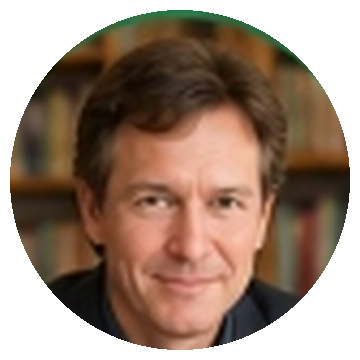
\includegraphics[width=2.06cm]{img_infografia/sawyer_photo.png}};

  \fill[infOrangeLight] (17.12,-3.04) rectangle (25.03,-2.56);
  \node[font=\fontsize{6.9}{8.0}\selectfont\bfseries\color{infOrange}] at (21.075,-2.80) {Personalización, conocimiento distribuido y lección TIMSS};

  \InfSectionBar{17.20}{-3.16}{infOrange}{infOrangeLight}{target}{Idea central del eje}
  \node[anchor=north west,text width=7.65cm,align=left,font=\fontsize{6.6}{8.0}\selectfont\color{infInk},inner sep=0pt] at (17.25,-3.74) {%
    Un aula rediseñada combina fuentes plurales, personalización sensible, colaboración intelectual, menor saturación temática y evaluación centrada en comprensión conceptual integrada.%
  };

  \InfSectionBar{17.20}{-4.86}{infOrange}{infOrangeLight}{key}{Conceptos clave}
  \InfConceptCard{17.20}{-5.44}{infOrange}{infOrangeCard}{personas}{\textbf{Saber distribuido}\\Equipos y herramientas reales.}
  \InfConceptCard{19.17}{-5.44}{infOrange}{infOrangeCard}{grafica}{\textbf{Lección TIMSS}\\Coherencia supera cobertura.}
  \InfConceptCard{21.14}{-5.44}{infOrange}{infOrangeCard}{doc}{\textbf{Evaluación real}\\Medir integración y sentido.}
  \InfConceptCard{23.11}{-5.44}{infOrange}{infOrangeCard}{balanza}{\textbf{Rol profesional}\\Docente diseñador y tutor.}

  \InfSectionBar{17.20}{-7.78}{infOrange}{infOrangeLight}{bulb}{Aportes principales}
  \InfBullet{17.22}{-8.38}{infOrange}{Estudios TIMSS prueban que planes saturados de temas superficiales logran menor desempeño matemático.}
  \InfBullet{17.22}{-9.04}{infOrange}{El maestro deja de ser única fuente de saber; coordina libros, simuladores, expertos y trabajo tutelado.}
  \InfBullet{17.22}{-9.70}{infOrange}{Las pruebas estandarizadas convencionales ignoran errores conceptuales profundos y desincentivan el proyecto.}
  \InfBullet{17.22}{-10.36}{infOrange}{Conectar escuela, museos, aprendizaje tutelado (\textit{apprenticeship}) y formación continua supera fronteras rígidas.}

  \InfSectionBar{17.20}{-11.12}{infOrange}{infOrangeLight}{gear}{Implicaciones en Matemáticas}
  \InfCheck{17.22}{-11.72}{infOrange}{Priorizar pocas familias de modelos estudiadas a profundidad.}
  \InfCheck{17.22}{-12.26}{infOrange}{Valorar coherencia entre tabla, gráfica, ecuación y texto.}
  \InfCheck{17.22}{-12.80}{infOrange}{Evaluar dictámenes técnicos por fases con retroalimentación.}
  \InfCheck{17.22}{-13.34}{infOrange}{Articular la autonomía del profesorado técnico en academia.}

  \fill[infOrangeLight,rounded corners=5pt] (17.20,-15.52) rectangle (24.95,-14.05);
  \node[text width=7.35cm,align=center,font=\fontsize{6.6}{8.1}\selectfont\color{infOrange}] at (21.075,-14.78) {%
    \textbf{\textit{«El profesorado debe actuar como trabajador del conocimiento, igual que médicos o ingenieros.»}}\\
    {\scriptsize — Eje sistémico · Sawyer (2008)}%
  };

  % PIE DE FUENTE Y CREDITOS
  \draw[fill=infGreen,draw=infGreen,rounded corners=6pt] (0.0,-16.92) rectangle (25.15,-15.88);
  \node[inner sep=0pt] at (0.72,-16.40) {\InfIconOutline[0.36]{libro}{white}};
  \node[anchor=west,text width=16.8cm,align=left,font=\fontsize{6.6}{8.0}\selectfont\color{white}] at (1.30,-16.40) {%
    \textbf{FUENTE BASE (APA 7):} Sawyer, R. K. (2008). Optimizing learning: Implications of learning sciences research. En OECD/CERI, \textit{Innovating to learn, learning to innovate} (cap. 2, pp. 45--65). OECD Publishing. \url{https://doi.org/10.1787/9789264039958-en}%
  };
  \node[anchor=east,text width=6.4cm,align=right,font=\fontsize{6.1}{7.4}\selectfont\color{white!90}] at (24.90,-16.40) {%
    \textbf{Mtro. Martín Jonathan de la Cruz Muñoz (Matrícula 00874)}\\
    IIIEPE · MAEM · Cohorte SD26 · Actividad 9 (Módulos 51436 / 51440)%
  };
\end{tikzpicture}}
\end{frame}

\begin{frame}{Mapa Infográfico de los Cinco Pilares de Sawyer (2008)}
  \centering
  \begin{tikzpicture}[scale=0.82, transform shape, font=\scriptsize, >=Latex]
    \node[draw=iiiepeNavy,fill=iiiepeNavy,text=white,rounded corners=4pt,text width=4.2cm,align=center,inner sep=5pt] (c) at (0,0) {\textbf{Ciencias del Aprendizaje}\\(Sawyer, 2008 · OECD/CERI)};
    \node[draw=iiiepeBlue,fill=iiiepePale,rounded corners=4pt,text width=3.9cm,align=left,inner sep=5pt] (n1) at (-4.8,2.1) {\textbf{1. Comprensión profunda}\\Conectar hechos y procedimientos en redes conceptuales transferibles.};
    \node[draw=iiiepeAqua!80!black,fill=iiiepeMint,rounded corners=4pt,text width=3.9cm,align=left,inner sep=5pt] (n2) at (4.8,2.1) {\textbf{2. Saberes previos activos}\\Visibilizar y reestructurar ideas y matemáticas ingenuas.};
    \node[draw=iiiepeOrange!90!black,fill=iiiepeWarm,rounded corners=4pt,text width=3.9cm,align=left,inner sep=5pt] (n3) at (-4.8,-2.1) {\textbf{3. Articulación y metacognición}\\Externalizar razonamientos y regular el espacio del problema.};
    \node[draw=iiiepeNavy,fill=iiiepePale,rounded corners=4pt,text width=3.9cm,align=left,inner sep=5pt] (n4) at (4.8,-2.1) {\textbf{4. Andamiaje y evaluación}\\Pistas graduadas que se retiran; evaluación para comprender.};
    \draw[->,very thick,iiiepeNavy] (c) -- (n1);
    \draw[->,very thick,iiiepeBlue] (c) -- (n2);
    \draw[->,very thick,iiiepeOrange!85!black] (c) -- (n3);
    \draw[->,very thick,iiiepeAqua!80!black] (c) -- (n4);
  \end{tikzpicture}
\end{frame}

\begin{frame}{Hallazgos Clave I: Comprensión Profunda y Saberes Previos}
  \begin{itemize}\normalsize
    \item \textbf{Base cognitiva del experto:} Poseer esquemas ricos y heurísticas adaptables ante situaciones cambiantes \textbf{(Sawyer, 2008)}.
    \item \textbf{Espacio del problema:} Antes de operar símbolos, comprender el contexto físico, las restricciones y el estado meta.
    \item \textbf{«Matemáticas ingenuas»:} El alumnado no entra como página en blanco; trae modelos intuitivos que la tarea debe hacer visibles.
    \item \textbf{Implicación en CONALEP/CECyTE:} Contrastar $y=kx$ frente a $y=mx+b$ antes de imponer fórmulas mecánicas.
  \end{itemize}
\end{frame}

\begin{frame}{Hallazgos Clave II: Articulación, Metacognición y Andamiaje}
  \begin{columns}[T]
    \column{0.48\textwidth}
      \begin{block}{Externalizar el pensamiento}
        \begin{itemize}\small
          \item Pensar en voz alta y justificar pasos consolida conceptos.
          \item La metacognición permite monitorear si la estrategia avanza hacia la meta.
          \item Articulación y comprensión forman un ciclo continuo.
        \end{itemize}
      \end{block}
    \column{0.48\textwidth}
      \begin{block}{Andamiaje efectivo (\textit{Scaffolding})}
        \begin{itemize}\small
          \item Apoyo temporal mediante pistas, tablas o contraejemplos.
          \item Hacer el ejercicio por el alumno anula el aprendizaje.
          \item Se agrega, ajusta y retira progresivamente conforme emerge autonomía.
        \end{itemize}
      \end{block}
  \end{columns}
\end{frame}

\begin{frame}{Principios para Diseñar Ambientes de Aprendizaje}
  \renewcommand{\arraystretch}{1.28}
  \scriptsize
  \begin{tabular}{p{3.4cm}p{5.2cm}p{4.8cm}}
    \toprule
    \textbf{Principio (Sawyer, 2008)} & \textbf{Contraste con modelo estándar} & \textbf{Aplicación en Matemáticas} \\
    \midrule
    Personalización & Todos ejecutan la misma guía al mismo ritmo. & Rutas escalonadas según diagnóstico previo. \\
    Fuentes diversas & Docente y libro único como autoridad absoluta. & Hojas de taller, sensores, simulaciones y textos. \\
    Conocimiento distribuido & Trabajo aislado individual sin consulta. & Equipos con roles de modelación y revisión. \\
    Currículo profundo (TIMSS) & Cobertura saturada y fragmentada por unidades. & Pocas familias de modelos con alta transferencia. \\
    Evaluación auténtica & Exámenes cerrados de memoria procedimental. & Dictámenes escritos y corrección formativa. \\
    \bottomrule
  \end{tabular}
\end{frame}

\begin{frame}{Transferencia Situada y Conclusiones}
  \begin{block}{Complementariedad con Philippe Meirieu (2020)}
    Meirieu aporta la finalidad ética y democrática de «hacer escuela y bien común»; Sawyer proporciona la ingeniería cognitiva y de ambientes que vuelve viable la comprensión profunda para todos.
  \end{block}
  \vspace{0.25cm}
  \begin{itemize}\normalsize
    \item Priorizar coherencia conceptual sobre acumulación fragmentada de fórmulas.
    \item Convertir la sala de matemáticas técnicas en taller de conjetura, prueba dimensional y argumentación.
  \end{itemize}
\end{frame}

\begin{frame}{Referencias (APA 7)}
  \scriptsize\setlength{\parskip}{5pt}
  \begin{itemize}
    \item Collin, J., y Quigley, A. (2021). \textit{Teacher feedback to improve pupil learning}. Education Endowment Foundation.
    \item Meirieu, P. (2020). ``La escuela después''... ¿Con la pedagogía de antes? \textit{MCEP}.
    \item Sawyer, R. K. (2008). Optimizing learning: Implications of learning sciences research. En \textit{Innovating to learn, learning to innovate} (pp. 45--65). OECD Publishing.
    \item Star, J. R., et al. (2015). \textit{Teaching strategies for improving algebra knowledge in middle and high school students}. IES.
  \end{itemize}
\end{frame}

\end{document}
